In questa sezione vengono brevemente introdotte le tecnologie utilizzate.

\section{Instant Developer}
La piattaforma web su cui è stato integrato il chatbot (\textit{Active Demand}) è stata sviluppata usando il framework di sviluppo \textbf{Instant Developer (In.de)} con cui Bookmark crea la maggior parte delle sue soluzioni software.

In.de è un proprio sistema di sviluppo con cui è possibile creare \textit{Rich Internet Application} e che nasce con l'obiettivo di ridurre i tempi di sviluppo, astranedo dai dettagli tecnici di basso livello, quali la scelta della specifica implementazione tecnologica sottostante, quindi disaccoppiando l'ambito applicativo da quello tecnologico.
%
Queste applicazioni sono poi automaticamente tradotte e compilate sia in linguaggio \texttt{Java} che \texttt{C\#}, in modo da funzionare su qualunque server. 

Una peculiarità di questo sistema di sviluppo è che è incentrato sulla programmazione relazionale: il codice non viene memorizzato in file di testo ma in un grafo le cui relazioni vengono tracciate dall'IDE. 
%
Questo dovrebbe sollevare, almeno in parte, stando agli intenti degli ideatori di In.de, il programmatore dal dover riadattare il software a fronte di cambiamenti nelle specifiche di progetto.

Le \textit{Rich Internet Application} sviluppate con In.de sono basate su un \textit{framework} il cui schema di funzionamento è riassunto nel diagramma di \Cref{fig:framework} e che contiene i moduli per la gestione delle connessioni con il \textit{database}, della rappresentazione logica dell'interfaccia utente, nonché quelli per l'applicazione dei profili applicativi, per la personalizzazione dell'applicazione e per il controllo dell'andamento della sessione. 
%
L'oggetto \textit{In memory database} visualizzato nella parte sinstra dello schema è parte del \textit{framework} che coordina la \textit{business logic} e il \textit{presentation manager}.

\begin{figure}
    \centering{}
    \includegraphics*[width=\textwidth]{./img/framework-inde.png}
    \caption{Framework In.de}
    \label{fig:framework}
\end{figure}

\section{Chatbot}
Il chatbot utilizzato è di tipo ad "oracolo".
%
La differenza sostanziale con un chatbot procedurale è che l'utente, nell'ultimo caso, è guidato, sin dall'inizio, a compiere un insieme di scelte che lo portano a seguire uno degli $n$ percorsi prefissati in fase di sviluppo, mentre un chatbot di tipo ad "oracolo" è addestrato a riconoscere ed interpretare il senso della frase scritta dall'utente e a rispondere in modo adeguato.
%
Questo ultimo approccio consentirebbe quindi, teoricamente, se configurato opportunamente, di poter rispondere a qualsiasi tipo di domanda o input dell'utente.

In \Cref{fig:chatbot-types} sono mostrati un esempio di \textit{chatbot} procedurale in cui è lo stesso \textit{chatbot} a guidare l'utente in uno dei possibili percorsi progettati (diventa cliente, stato attivazione, guasto di linea, fattura, ...) e un esempio di \textit{chatbot} ad "oracolo" in cui il chatbot si pone in ascolto dell'input dell'utente e cerca di riconoscere, attraverso l'analisi sintattica e semantica della frase, quale sia l'intento dell'utente.

\begin{figure}
    \centering{}
    \subfloat[\centering Esempio di chatbot procedurale - TOBi (Vodafone) ]{{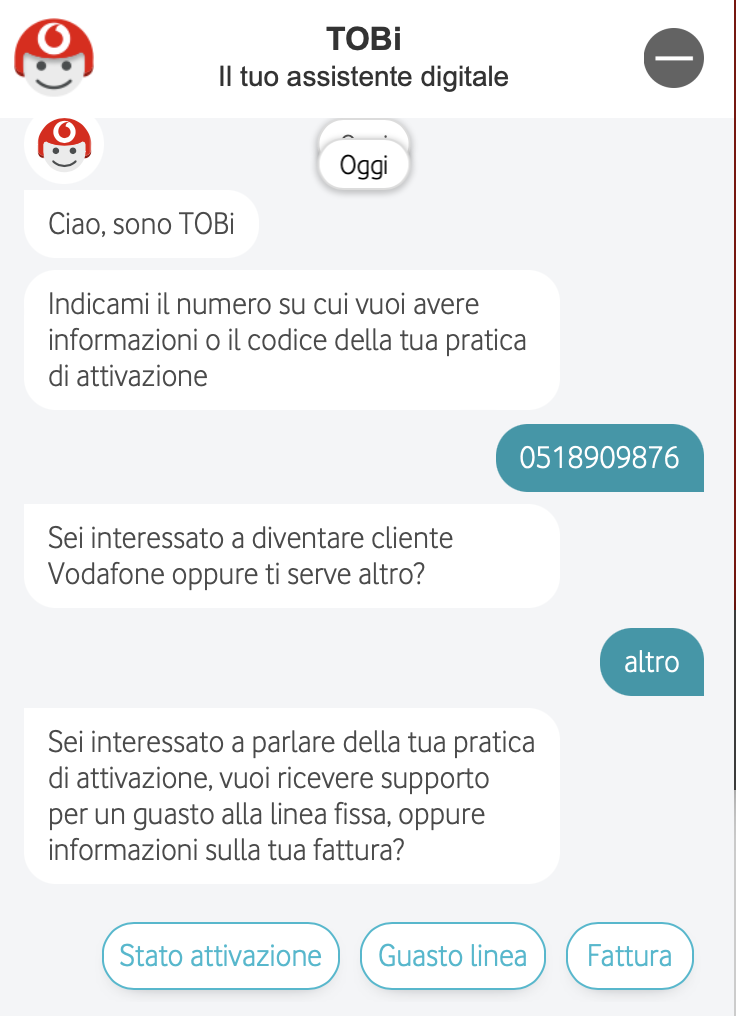
\includegraphics[width=5.9cm]{./img/chatbot-procedurale.png} }}
    \qquad
    \subfloat[\centering Esempio di chatbot ad "oracolo"]{{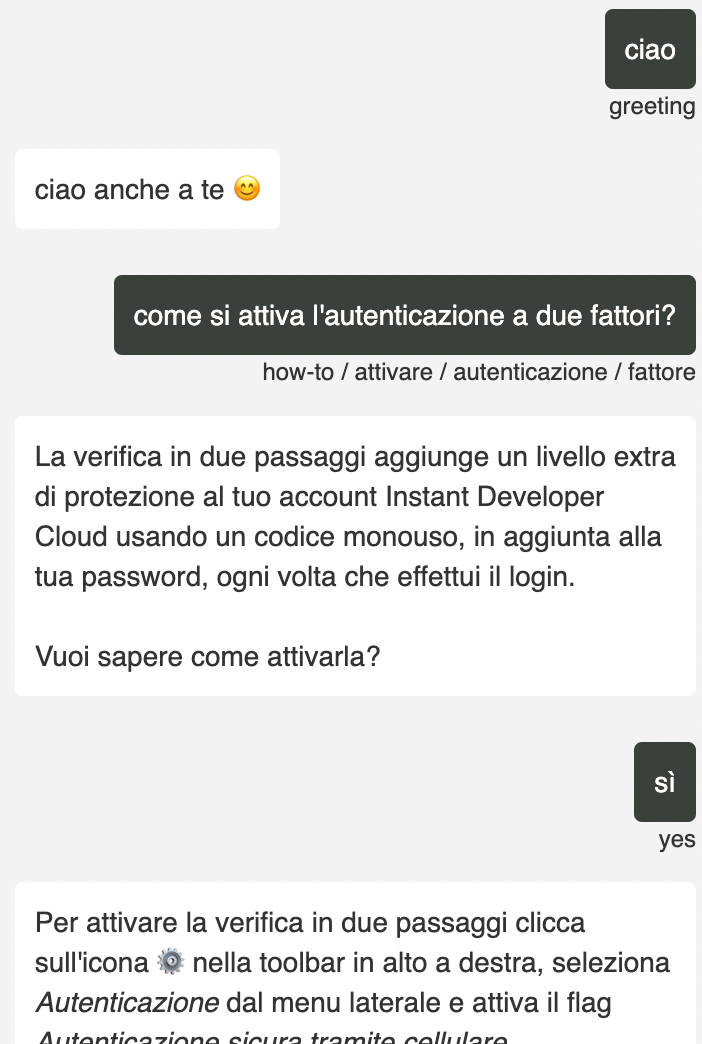
\includegraphics[width=5.7cm]{./img/chatbot-oracolo.png} }}
    \caption{Esempi di chatbot}
    \label{fig:chatbot-types}
\end{figure}

Il funzionamento del chatbot si basa sul riconoscimento e l'interpretazione dei messaggi scritti dall'utente, sfruttando il servizio \textit{Google NLP}, una tecnologia in grado di generare, grazie all'utilizzo dell'IA, l'albero semantico relativo alla frase scritta dell'utente e confrontarlo con ciascuno degli alberi semantici con cui è stato configurato.

\textit{Instant Support Editor} è l'applicazione web per la gestione e configurazione di tutto ciò che concerne il cuore del chatbot: dalla scrittura delle definizioni, al concepimento dei flussi.
%
A questa applicazione è poi affiancata un'applicazione (web e \textit{mobile}) che consente agli operatori di interloquire con l'utente.

